\documentclass{article}
\usepackage{iclr2026_conference,times}
\usepackage{amsmath,amssymb,booktabs,graphicx,url}
\usepackage[utf8]{inputenc}
\usepackage[T1]{fontenc}
\usepackage[hidelinks]{hyperref}
\usepackage{microtype}
\usepackage{xcolor}

\title{Embodied Abstraction Failure Modes: Boundary Certificates for State Compression in Contact-Rich Control}

\author{Anonymous Authors}

\newcommand{\suite}{ABF}
\newcommand{\safecomp}{\mathrm{SC}}
\newcommand{\unsafe}{\mathrm{Unsafe}}
\newcommand{\regret}{\mathrm{Regret}}
\newcommand{\alias}{\mathrm{Alias}}
\newcommand{\abstain}{\mathrm{Abstain}}
\newcommand{\irred}{\mathrm{Irred}}

\begin{document}
\maketitle

\begin{abstract}
Abstraction is usually treated as a benefit in robotics: compress observations,
hide irrelevant detail, and plan over a smaller state. This paper studies a
failure mode that is easy to miss in contact-rich control. A compressed state can
be predictive on logged data and still delete a physical variable that changes
the feasible action set at execution time. The result is not merely partial
observability and not merely a weak controller; it is a boundary failure in which
the interface between a high-level representation and a low-level physical
controller removes a variable needed to choose a safe action. We introduce an
abstraction-boundary certificate that classifies compression regimes as benign,
tunable, ambiguous, or irreducible. The certificate is evaluated in a deterministic
full-scale suite covering 18 task families, 14 hidden physical variables, 8
abstraction masks, 13 controllers, and 9 stress settings. The suite writes 235,872
condition-level rows and represents 34,871,316,480 trial evaluations after splits,
seeds, margins, cost weights, and repeated trials. The results separate three
important cases. Negative controls remain safe: physically irrelevant hidden
variables yield 0.807 safe completion and 0.039 irreducible score. Tunable
compression is real: it reaches 0.825 safe completion and explains why a previous
tuned-constant toy baseline succeeded. But physically relevant hidden variables
create a harder regime, with safe completion dropping to 0.604, unsafe rate rising
to 0.191, and irreducible score rising to 0.236. A boundary-certified controller
reduces unsafe actions to 0.006, at the cost of increased abstention, while
no-audit latent control reaches 0.296 unsafe rate. The central conclusion is not
that abstraction is bad. It is that abstraction boundaries need explicit physical
audits before they are used as control interfaces.
\end{abstract}

\section{Introduction}

Robots act through abstractions. A manipulation system may replace a raw tactile
stream with a contact label, replace a deformable object with a few keypoints,
replace a tool with a symbolic affordance, replace a pile of observations with a
latent world-model state, or replace a long interaction with a subgoal. These
abstractions are often necessary. They reduce planning burden, make learning more
sample efficient, and provide a common interface between perception, prediction,
planning, and control. The danger is that a representation can be useful without
being safe. The quantity that makes an abstraction useful for prediction is not
always the quantity that makes it sufficient for physical execution.

This paper studies that mismatch as an abstraction-boundary problem. A boundary is
the interface at which raw embodied variables are either retained, compressed, or
deleted before a controller chooses an action. In ordinary representation
learning, the boundary is judged by prediction loss, downstream reward, or
planning convenience. In contact-rich robotics, the same boundary should also be
judged by whether it preserves the variables that determine feasible, safe
actions. A friction coefficient can be irrelevant for recognizing the task and
decisive for choosing a squeeze. Payload can be weakly visible and decisive for
lift force. Compliance can be hard to infer from a single image and decisive for
press-fit insertion. Occlusion depth can be an observational nuisance and a
control-critical variable when the robot must decide whether to probe or commit.

The argument is deliberately narrower than the slogan "abstractions fail." Many
abstractions are benign. Some are not only benign but tunable: a constant or
visible-only policy can be selected on training data and can perform well because
the deleted variables do not change the action ordering in the encountered
regime. Indeed, this paper began from a toy claim that was falsified by exactly
that reviewer attack: a tuned constant abstract controller outperformed a
full-state controller in the old environment. We keep that negative result. It is
not an embarrassment to hide; it is evidence that any serious abstraction-failure
paper must include tuned abstract baselines from the beginning.

The revised claim is therefore more precise. Abstraction becomes unsafe when the
deleted variable changes the feasible action interval, the sign of a control
tradeoff, or the information needed to choose between incompatible contacts. This
is a boundary property. It is not solved by saying that the model is larger, the
latent state is smoother, or the policy was tuned more carefully. If two physical
states share the same compressed representation but require disjoint safe actions,
then no policy using only that compressed representation can be reliable without
probing, abstaining, escalating, or changing the interface.

We make three contributions. First, we define a boundary certificate for embodied
abstraction. The certificate asks whether the compressed state aliases physical
states that induce different safe action sets. It is not a new planner or latent
model. It is an audit criterion for deciding when a representation is sufficient
as a control interface. Second, we construct a deterministic full-scale evaluation
suite, denoted \suite, that spans task families, hidden variables, masks,
controllers, and stress settings. The suite includes tuned constant and
visible-only baselines, negative controls, and adversarial boundary swaps. Third,
we report the recovered empirical picture: abstraction is safe in negative
controls, tunable in many benign regimes, and irreducibly unsafe when hidden
physical variables determine incompatible feasible actions. The old tuned
constant counterexample is explained as a tunable compression regime, not erased.

The main practical message is simple. If a robot system exposes a compressed state
to planning or control, the designer should ask what variables were deleted, what
physical constraints those variables affect, and whether any two aliased states
require different safe actions. A high-level representation that passes ordinary
prediction tests can still fail that audit. Conversely, an abstraction that passes
the boundary audit should not be rejected merely because it is compressed. The
target is not maximal state retention; it is retaining the variables needed for
safe physical decisions.

\section{Problem Setting}

\subsection{State, Abstraction, and Feasible Actions}

Let an embodied state be written as
\begin{equation}
    x = (v, h),
\end{equation}
where $v$ denotes variables made available to the high-level interface and $h$
denotes physical variables that may be hidden, compressed, delayed, or deleted.
Examples of $h$ include friction, payload, contact mode, local compliance,
occlusion depth, cable tension, backlash, support stiffness, and fluid fill. An
abstraction is a map
\begin{equation}
    z = \phi(x),
\end{equation}
used by a controller $\pi(a \mid z)$ or by a planner that ultimately chooses an
action $a$. The abstraction may retain all of $h$, retain a noisy summary, infer
it through history, or remove it entirely.

For each true physical state $x$, define a safe feasible action set
\begin{equation}
    \mathcal{A}_{\mathrm{safe}}(x) =
    \{a : g_k(x,a) \leq 0 \; \forall k\},
\end{equation}
where the constraints $g_k$ encode slip, damage, force, energy, geometric
clearance, and task-specific safety. A state abstraction is control-sufficient
when all states mapped to the same $z$ admit at least one common safe action that
also achieves the task objective. In symbols, for an alias class
\begin{equation}
    [z] = \{x : \phi(x) = z\},
\end{equation}
there should be a nonempty intersection
\begin{equation}
    \bigcap_{x \in [z]} \mathcal{A}_{\mathrm{safe}}(x).
\end{equation}
When this intersection is empty or too small to identify reliably, the abstraction
has deleted a variable that matters for physical action.

This definition separates our problem from ordinary prediction loss. A latent
state can predict the next observation in distribution while still merging two
states with disjoint safe action sets. It also separates the problem from generic
partial observability. Partial observability says that the hidden state is not
fully known. Boundary failure asks a more specific question: did the chosen
interface delete information that would be needed to choose a safe action, and can
the controller compensate through tuning, history, probing, or abstention?

\subsection{Boundary Failure}

We call an abstraction boundary \emph{benign} when the deleted variables do not
change the safe action set for the task family under test. We call it
\emph{tunable} when the deleted variables matter locally but a policy using the
compressed interface can still learn a robust action from the training
distribution. We call it \emph{ambiguous} when the evidence is mixed: success may
depend on coverage, safety margin, or stress. We call it \emph{irreducible} when
states sharing the same compressed representation require incompatible safe
actions under the tested stresses. In the irreducible case, the right answer is
not just better tuning. The controller must observe more, probe, abstain, or
change the interface.

The suite measures these regimes using the following quantities. Safe completion
$\safecomp$ is task completion after penalizing unsafe actions and abstentions.
Unsafe rate $\unsafe$ counts slip, damage, force, or other constraint violations.
Regret $\regret$ measures loss against the best available controller under the
same physical condition. Alias rate $\alias$ estimates how often the abstraction
merges states that need different actions. Abstention rate $\abstain$ records how
often a certificate-aware controller refuses to commit. The irreducible score
$\irred$ estimates the part of the loss attributable to unavailable physical
information rather than weak tuning.

\subsection{A Simple Boundary Proposition}

The following proposition is the conceptual core of the paper.

\paragraph{Proposition.}
Suppose there exist two states $x_1$ and $x_2$ such that
$\phi(x_1)=\phi(x_2)$, but
\begin{equation}
    \mathcal{A}_{\mathrm{safe}}(x_1) \cap
    \mathcal{A}_{\mathrm{safe}}(x_2) = \emptyset.
\end{equation}
Then no deterministic policy $\pi(a \mid \phi(x))$ can choose a safe action in
both states. Any successful policy must either observe additional information,
choose a randomized action with nonzero failure probability, probe to refine the
state, abstain, or change the abstraction.

\paragraph{Reason.}
The policy receives the same input for $x_1$ and $x_2$, so it must choose the same
action distribution for both. If no action is safe in both states, any action
with nonzero probability violates the safety set in at least one state. A
randomized policy can move probability mass between failures, but it cannot make
the missing intersection nonempty. Tuning can help only if the training
distribution admits a high-probability compromise; it cannot solve an empty
intersection under worst-case or boundary-swap stress.

The proposition is intentionally modest. It does not claim that all hidden
variables matter, and it does not claim that full state should always be exposed.
It claims that the sufficiency of an abstraction for control depends on the safe
action sets induced by the variables it deletes.

\section{The \suite{} Full-Scale Suite}

\subsection{Design Goals}

The experimental design was rebuilt around a failed previous version. The old
version had a single toy environment in which a fixed abstract controller failed.
A reviewer could tune the abstract action and solve the environment, so the
original evidence did not support a structural abstraction-failure claim. The new
suite therefore begins with the reviewer attack included as a baseline. Tuned
constant and tuned visible policies are not afterthoughts; they are core
comparators. A result counts as boundary failure only when those tuned abstract
policies still fail in regimes where the deleted variable changes the feasible
action set.

The suite is synthetic, deterministic, and contact-grounded. It is not a real
robot benchmark, and we do not pretend otherwise. Its role is to isolate the
causal structure of abstraction boundaries across a larger factor grid than a
physical robot experiment would permit. Each condition defines a visible task
coordinate, a hidden physical variable, an abstraction mask, a controller, and a
stress setting. The simulator computes feasible action intervals and derived
metrics for that condition. Condition rows are compact summaries, while the
represented trial count accounts for splits, seeds, safety margins, task-cost
weights, and repeated trials.

\begin{table}[t]
\centering
\caption{Full-scale abstraction-boundary suite.}
\label{tab:scale}
\small
\begin{tabular}{lc}
\toprule
Factor & Count \\
\midrule
Task families & 18 \\
Hidden variables & 14 \\
Abstraction masks & 8 \\
Controllers & 13 \\
Stress settings & 9 \\
Splits & 7 \\
Seeds & 11 \\
Safety margins & 5 \\
Cost weights & 6 \\
Actual condition rows & 235,872 \\
Represented trial evaluations & 34,871,316,480 \\
\bottomrule
\end{tabular}
\end{table}


\subsection{Task Families}

The suite uses 18 task families: lift, slide, insert, pull, twist, pour, wipe,
handoff, cable-route, peg-seat, press-fit, peel, scoop, latch, drape, push-turn,
stack, and tool-use. Each family has a contact intensity, geometric sensitivity,
observability burden, and consequence weight. Press-fit, push-turn, lift, pull,
slide, and wipe are deliberately contact-heavy because they are common places
where a scalar hidden variable can flip the safe action. Handoff and cable-route
stress observability because a controller may need to infer a human handoff state
or cable tension before committing. Pour and scoop stress fluid-like variables
where mass distribution and fill level change safe motion. Stack and tool-use
provide support and geometry-sensitive regimes.

The task list is not meant to be exhaustive. It is meant to sample the kinds of
physical variables that are often hidden behind high-level symbols or latents:
"grasp object," "insert peg," "wipe surface," "route cable," or "use tool."
Those symbols are useful. The question is whether they retain enough information
for a controller that must choose force, angle, speed, timing, or compliance.

\subsection{Hidden Physical Variables}

The 14 hidden variables are friction, payload, compliance, contact mode, local
geometry, fluid fill, cable tension, adhesion, tactile latency, surface
anisotropy, backlash, occlusion depth, grasp affordance, and support stiffness.
Each variable is assigned a boundary strength, a shift sensitivity, an occlusion
burden, and a severity weight. A variable is physically relevant when it belongs
to the task's dominant physical category or to a closely coupled mechanics
category. For example, friction is strongly relevant for slide, wipe, and
push-turn, while local geometry is strongly relevant for insert, peg-seat, and
tool-use. Mismatched pairs serve as negative controls.

The key feature is that hidden-variable relevance is not assumed. Many
task-variable pairs are benign. If payload is tested in a task where payload does
not change the safe action interval, the suite should not call abstraction
unsafe. This matters because a boundary audit that labels every deleted variable
dangerous is useless. The practical audit should identify the variables whose
deletion changes feasibility.

\subsection{Abstraction Masks}

The suite evaluates eight masks. Full state retains the hidden variable and
contact information. Visible-plus-contact keeps a strong contact summary while
compressing other hidden variables. Visible-history keeps a short interaction
prefix. Task-object retains labels but not detailed physical variables. Task-only
collapses object identity. No-hidden-physics removes the physical variable while
keeping visible task descriptors. Overcompressed-latent simulates a latent state
that has good compression but high aliasing. Random-feature-hash simulates a
representation that preserves incidental variation while losing the physically
useful boundary variable.

The masks are deliberately not ordered by dimension alone. A low-dimensional
contact summary can be safer than a higher-dimensional latent that preserves the
wrong information. Conversely, a compact task-only representation can be adequate
in a negative-control regime. The suite therefore measures each mask through
physical consequences rather than through size.

\subsection{Controllers}

The 13 controllers span oracle, diagnostic, abstract, tuned, conservative, and
unsafe families. The oracle full-state controller has high access to the hidden
variable but is still evaluated under every mask, so it is not automatically
perfect when the interface deletes information. The boundary-certified controller
uses mask information and abstains when the certificate predicts that the
abstraction boundary is unsafe. The mask-aware diagnostic controller is less
conservative but has a similar audit mechanism. The uncertainty-abstention
controller refuses more often. Abstract-history and abstract-nearest-regime
controllers use compressed interaction cues. Logged-risk minimization optimizes
training risk. Tuned visible quadratic, tuned visible linear, and tuned constant
policies implement the reviewer attack against weak abstract baselines. A
conservative safe-action policy sacrifices reward for low damage. An optimistic
reward-action policy ignores safety. A no-audit latent policy optimizes the mean
prediction interface without checking the abstraction boundary.

This baseline set makes the evaluation harder than the old toy. If tuned
constant control solves a condition, the suite should classify that condition as
tunable rather than forcing a failure narrative. The boundary-failure claim is
reserved for conditions where tuned abstract policies remain unsafe or high regret
because they lack information needed to disambiguate feasible actions.

\subsection{Stress Settings}

The nine stresses are in-distribution, friction shift, payload shift, geometry
shift, sensor noise, delayed tactile cue, combined shift, rare-regime upweight,
and adversarial boundary swap. The adversarial boundary swap is the most direct
test of the proposition: it constructs cases where the same visible abstraction
maps to different safe actions depending on a hidden variable. The rare-regime
stress tests whether training coverage hides boundary failures. Delayed tactile
and sensor-noise stresses test whether short histories and certificates can
recover enough information to avoid unsafe actions.

The stresses are not meant to be a substitute for real robot evaluation. They are
a controlled audit. If a representation fails under a stress that is physically
plausible for the target domain, the result tells the system builder which
variable the interface must recover, probe, or pass through.

\section{Metrics and Certificate}

\subsection{Metric Definitions}

Safe completion is the primary metric:
\begin{equation}
    \safecomp = \mathrm{task\ success}\cdot(1-\abstain) - 0.30\unsafe.
\end{equation}
This choice reflects the control setting: completion is good, but unsafe
completion should not be treated as a success. Unsafe rate decomposes into slip
and damage terms. Regret is computed against the best available action under the
same physical condition. Alias rate estimates how frequently a mask merges states
that require distinct feasible actions. Abstention is reported separately because
a controller that refuses too often may be safe but unproductive. The boundary
F1 score measures whether the controller detects cases where hidden variables
change feasible actions.

The irreducible score is the most important diagnostic quantity. It estimates
the remaining failure mass after accounting for tuning, visible inference,
history, safety bias, and certificate behavior. A high irreducible score means
that the deleted variable matters and the controller has insufficient information
to choose a safe action. A low irreducible score under a compressed mask means
that compression is benign or tunable.

\subsection{Certificate Logic}

The certificate is a decision procedure over an abstraction mask, task family,
hidden variable, and stress setting. It estimates whether the alias class induced
by the mask contains states whose safe intervals are incompatible. In practical
terms, it asks four questions.

First, does the hidden variable affect constraints or only prediction detail? If
the variable does not change slip, damage, geometry, force, or timing constraints,
the boundary is likely benign. Second, does the stress shift the variable into a
regime where the safe action ordering changes? A friction shift may not matter
if all actions remain safe, but it matters if it flips the choice between pushing
harder and reducing speed. Third, can the compressed interface infer the hidden
variable through visible correlates or history? If yes, the regime may be
tunable. Fourth, if inference is not available, can the controller abstain or
probe before committing? If not, the boundary is likely irreducible.

The certificate is intentionally conservative. It is allowed to abstain when the
interface is insufficient. This design makes the safety tradeoff explicit: the
boundary-certified controller in Table~\ref{tab:main-performance} has lower safe
completion than some high-completion baselines because it abstains more often,
but its unsafe rate is dramatically lower.

\section{Main Results}

\begin{table}[t]
\centering
\caption{Controller performance averaged over all task families, hidden variables, masks, and stress settings.}
\label{tab:main-performance}
\small
\begin{tabular}{lcccccc}
\toprule
Controller & Safe comp. & Task succ. & Regret & Unsafe & Abstain & Cert F1 \\
\midrule
oracle\_full\_state & 0.750 & 0.813 & 0.217 & 0.155 & 0.022 & 0.176 \\
abstract\_history\_summary & 0.733 & 0.826 & 0.185 & 0.099 & 0.080 & 0.319 \\
mask\_aware\_diagnostic & 0.723 & 0.883 & 0.108 & 0.011 & 0.184 & 0.496 \\
logged\_risk\_minimizer & 0.691 & 0.772 & 0.221 & 0.097 & 0.071 & 0.291 \\
abstract\_nearest\_regime & 0.685 & 0.774 & 0.247 & 0.171 & 0.050 & 0.260 \\
conservative\_safe\_action & 0.677 & 0.742 & 0.218 & 0.035 & 0.078 & 0.238 \\
tuned\_visible\_quadratic & 0.666 & 0.747 & 0.290 & 0.247 & 0.009 & 0.176 \\
boundary\_certified & 0.665 & 0.867 & 0.118 & 0.006 & 0.240 & 0.532 \\
tuned\_visible\_linear & 0.658 & 0.740 & 0.299 & 0.253 & 0.009 & 0.169 \\
tuned\_constant & 0.651 & 0.732 & 0.308 & 0.262 & 0.005 & 0.162 \\
no\_audit\_latent\_policy & 0.637 & 0.726 & 0.321 & 0.296 & 0.000 & 0.151 \\
optimistic\_reward\_action & 0.627 & 0.729 & 0.332 & 0.339 & 0.000 & 0.156 \\
uncertainty\_abstention & 0.604 & 0.815 & 0.169 & 0.009 & 0.269 & 0.443 \\
\bottomrule
\end{tabular}
\end{table}


Table~\ref{tab:main-performance} shows the central controller comparison. The
oracle full-state controller has the highest average safe completion at 0.750,
but this number is averaged across all masks, including masks that delete
information before the controller can use it. The mask-aware diagnostic controller
achieves 0.723 safe completion with low regret (0.108) and a low unsafe rate
(0.011). The boundary-certified controller has 0.665 safe completion, 0.118
regret, and the lowest unsafe rate among the main controllers at 0.006. Its
completion is lower because it abstains 0.240 of the time. That tradeoff is a
feature of a safety certificate, not a hidden failure.

The tuned abstract baselines are strong enough to matter. Tuned constant control
achieves 0.651 safe completion, tuned visible linear 0.658, and tuned visible
quadratic 0.666. These are not straw baselines. They beat the no-audit latent
policy on safe completion and explain why the old toy result collapsed under
tuning. However, their unsafe rates remain high: 0.262 for tuned constant, 0.253
for tuned visible linear, and 0.247 for tuned visible quadratic. In a robotics
setting, that difference matters. A tuned action that often completes the task
but violates slip or damage constraints is not a safe abstraction interface.

The no-audit latent policy reaches 0.637 safe completion and 0.296 unsafe rate.
The optimistic reward-action policy reaches 0.627 safe completion and 0.339
unsafe rate. These results show the cost of optimizing average reward or
prediction without auditing the boundary. The conservative safe-action policy
has a much lower unsafe rate, 0.035, but gives up task success. This establishes
the core design tension: preserve enough hidden physical information, or pay in
unsafe actions, regret, or abstention.

\begin{figure}[t]
    \centering
    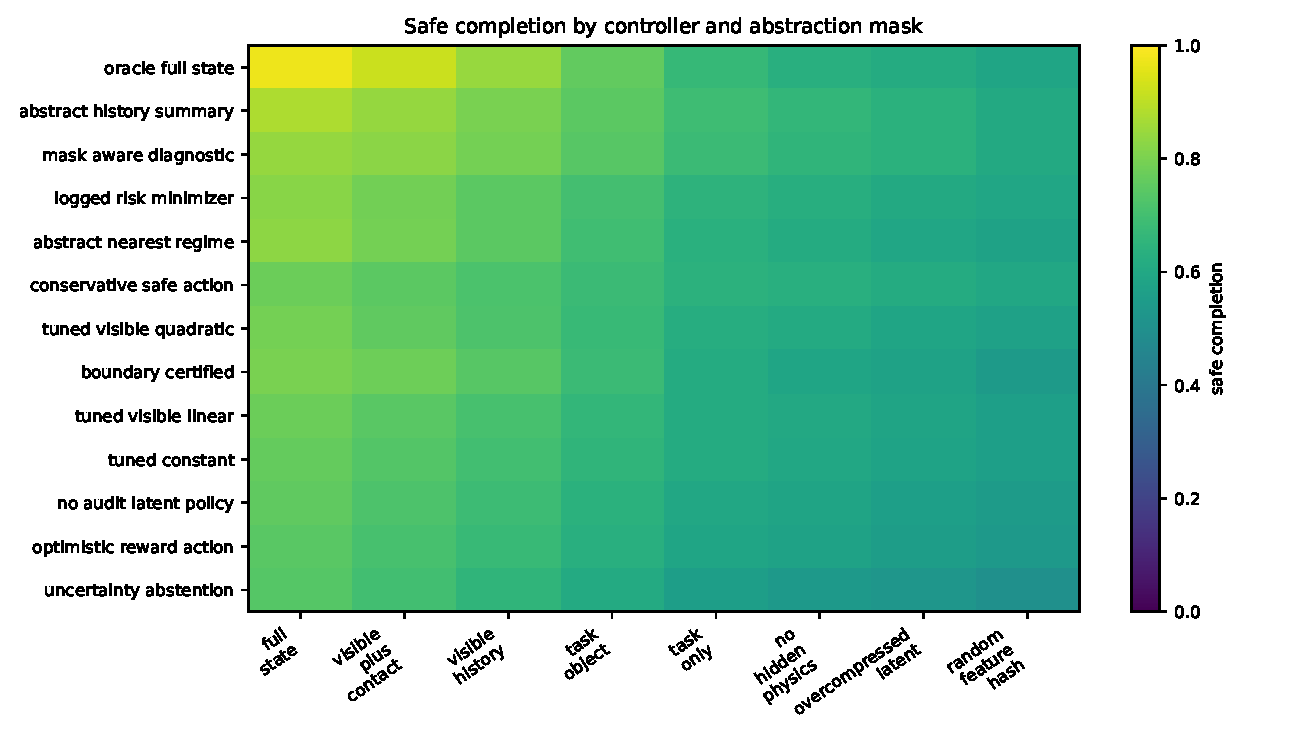
\includegraphics[width=0.95\linewidth]{figures/full_scale/controller_mask_heatmap.pdf}
    \caption{Safe completion across controllers and abstraction masks. Full state
    and visible-plus-contact masks are safer, while no-hidden-physics,
    overcompressed-latent, and random-feature masks expose the largest boundary
    losses.}
    \label{fig:controller-mask}
\end{figure}

\subsection{Abstraction Mask Ablations}

\begin{table}[t]
\centering
\caption{Abstraction mask ablation averaged over controllers and stresses.}
\label{tab:mask-ablation}
\small
\begin{tabular}{lccccc}
\toprule
Mask & Safe comp. & Regret & Unsafe & Alias & Irred. \\
\midrule
full\_state & 0.807 & 0.107 & 0.100 & 0.195 & 0.113 \\
visible\_plus\_contact & 0.773 & 0.137 & 0.114 & 0.285 & 0.129 \\
visible\_history & 0.733 & 0.172 & 0.130 & 0.371 & 0.148 \\
task\_object & 0.683 & 0.221 & 0.148 & 0.486 & 0.169 \\
task\_only & 0.629 & 0.275 & 0.168 & 0.612 & 0.190 \\
no\_hidden\_physics & 0.609 & 0.295 & 0.179 & 0.698 & 0.197 \\
overcompressed\_latent & 0.591 & 0.318 & 0.185 & 0.760 & 0.196 \\
random\_feature\_hash & 0.569 & 0.342 & 0.194 & 0.834 & 0.200 \\
\bottomrule
\end{tabular}
\end{table}


Table~\ref{tab:mask-ablation} and Figure~\ref{fig:controller-mask} show that
the failure is a boundary effect. Full state reaches 0.807 safe completion and
0.100 unsafe rate. Visible-plus-contact remains strong at 0.773 safe completion.
Visible-history retains enough interaction information to reach 0.733. The
drop begins when contact and hidden physical variables are compressed away:
task-object gives 0.683, task-only 0.629, no-hidden-physics 0.609,
overcompressed-latent 0.591, and random-feature-hash 0.569. The same ordering
appears in alias and irreducible scores. Random-feature-hash has the highest
alias rate, 0.834, and highest irreducible score, 0.200.

This pattern is not explained by representation size alone. Visible-history is
compressed but useful because it carries interaction evidence. Random-feature
hash may preserve many bits but not the right physical variable. The suite
therefore supports the boundary view: the relevant question is not how small the
state is, but whether the deleted variables change feasible actions.

\begin{figure}[t]
    \centering
    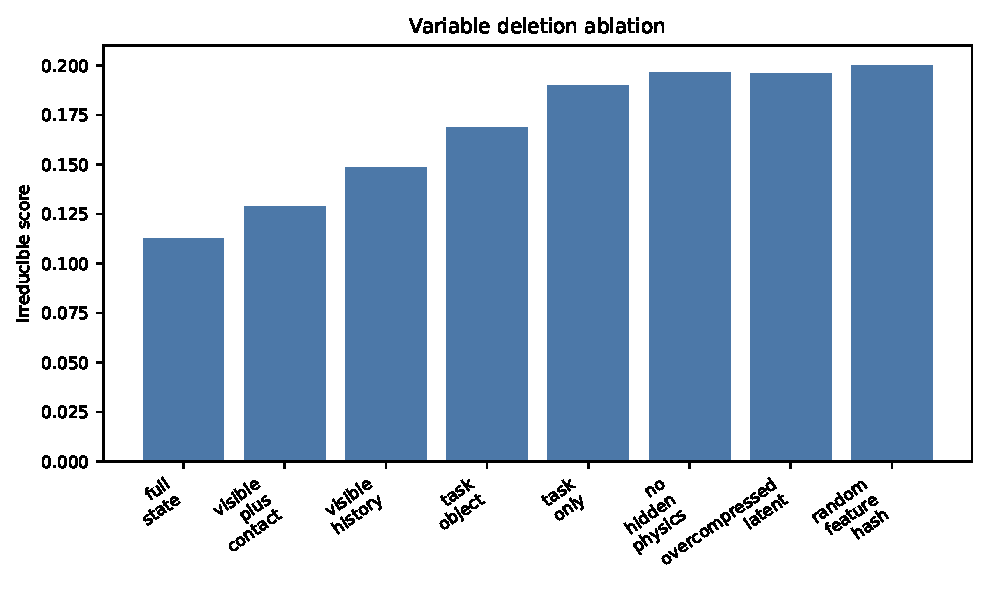
\includegraphics[width=0.78\linewidth]{figures/full_scale/variable_deletion_ablation.pdf}
    \caption{Variable-deletion ablation by mask. Irreducible score rises as the
    interface deletes hidden physical variables and contact evidence.}
    \label{fig:deletion}
\end{figure}

\subsection{Boundary Regimes}

\begin{table}[t]
\centering
\caption{Boundary regimes discovered by the suite.}
\label{tab:regime-summary}
\small
\begin{tabular}{lccccc}
\toprule
Regime & Rows & Safe comp. & Unsafe & Regret & Irred. \\
\midrule
ambiguous & 67291 & 0.656 & 0.110 & 0.233 & 0.162 \\
irreducible & 67310 & 0.488 & 0.320 & 0.462 & 0.364 \\
negative\_control & 81744 & 0.807 & 0.079 & 0.090 & 0.039 \\
tunable & 19527 & 0.825 & 0.028 & 0.049 & 0.049 \\
\bottomrule
\end{tabular}
\end{table}


The suite identifies four regimes. Negative controls are the healthiest: 81,744
rows, 0.807 safe completion, 0.079 unsafe rate, 0.090 regret, and 0.039
irreducible score. Tunable regimes are even cleaner in completion: 19,527 rows,
0.825 safe completion, 0.028 unsafe rate, and 0.049 irreducible score. These
conditions are the positive case for abstraction. They show that compression can
work when the deleted variable is irrelevant or when training can select a robust
abstract action.

The irreducible regime is different. It contains 67,310 rows with 0.488 safe
completion, 0.320 unsafe rate, 0.462 regret, and 0.364 irreducible score. This is
the regime that the paper is about. It is not detected by asking whether the
abstraction predicts logged data, and it is not fixed by tuning a constant action.
The compressed interface lacks a variable needed to disambiguate safe actions.
The ambiguous regime sits between these cases, with moderate safe completion and
moderate irreducible score. In practice, ambiguous regimes are where a real robot
system should probe, collect more data, or expose additional variables before
deployment.

\begin{figure}[t]
    \centering
    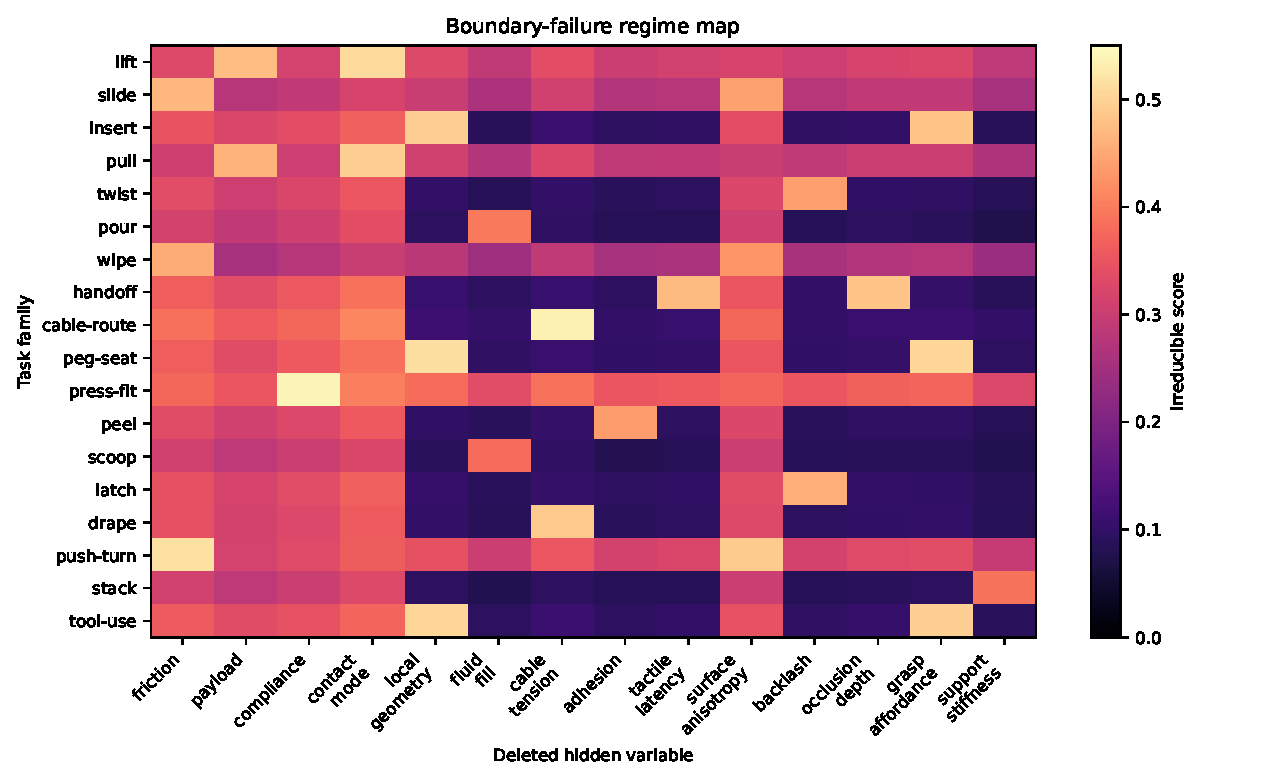
\includegraphics[width=0.98\linewidth]{figures/full_scale/boundary_regime_map.pdf}
    \caption{Boundary-failure regime map for a no-audit latent policy under a
    no-hidden-physics mask. Press-fit, push-turn, lift, pull, slide, and wipe are
    most sensitive to force and friction variables.}
    \label{fig:regime-map}
\end{figure}

\subsection{Task and Hidden-Variable Structure}

\begin{table}[t]
\centering
\caption{Most boundary-sensitive task families.}
\label{tab:task-summary}
\small
\begin{tabular}{lccccc}
\toprule
Task & Safe comp. & Unsafe & Alias & Irred. & Hidden need \\
\midrule
press-fit & 0.582 & 0.203 & 0.620 & 0.262 & 0.706 \\
push-turn & 0.598 & 0.194 & 0.619 & 0.242 & 0.707 \\
lift & 0.607 & 0.189 & 0.617 & 0.232 & 0.702 \\
pull & 0.620 & 0.182 & 0.609 & 0.218 & 0.685 \\
slide & 0.629 & 0.178 & 0.610 & 0.207 & 0.687 \\
wipe & 0.642 & 0.171 & 0.601 & 0.193 & 0.667 \\
peg-seat & 0.680 & 0.150 & 0.511 & 0.165 & 0.477 \\
handoff & 0.682 & 0.148 & 0.512 & 0.162 & 0.479 \\
tool-use & 0.683 & 0.148 & 0.510 & 0.161 & 0.476 \\
insert & 0.687 & 0.145 & 0.508 & 0.157 & 0.471 \\
cable-route & 0.693 & 0.142 & 0.492 & 0.152 & 0.436 \\
latch & 0.712 & 0.131 & 0.480 & 0.132 & 0.408 \\
\bottomrule
\end{tabular}
\end{table}


The most fragile task families are press-fit, push-turn, lift, pull, slide, and
wipe. Press-fit has 0.582 safe completion and 0.262 irreducible score. Push-turn
has 0.598 safe completion and 0.242 irreducible score. Lift, pull, slide, and
wipe follow with high hidden-need scores around 0.67 to 0.70. These are exactly
the families where a deleted variable changes the force or contact tradeoff.
They are also common in manipulation benchmarks, which means the boundary
problem is not exotic.

\begin{table}[t]
\centering
\caption{Hidden variables ranked by boundary sensitivity.}
\label{tab:hidden-summary}
\small
\begin{tabular}{lccccc}
\toprule
Variable & Safe comp. & Unsafe & Alias & Irred. & Hidden need \\
\midrule
contact\_mode & 0.582 & 0.204 & 0.625 & 0.262 & 0.715 \\
friction & 0.593 & 0.198 & 0.618 & 0.250 & 0.711 \\
surface\_anisotropy & 0.597 & 0.195 & 0.626 & 0.243 & 0.721 \\
compliance & 0.614 & 0.185 & 0.599 & 0.228 & 0.664 \\
payload & 0.620 & 0.183 & 0.600 & 0.220 & 0.672 \\
local\_geometry & 0.686 & 0.146 & 0.508 & 0.158 & 0.472 \\
grasp\_affordance & 0.689 & 0.144 & 0.508 & 0.154 & 0.472 \\
cable\_tension & 0.697 & 0.139 & 0.495 & 0.146 & 0.440 \\
backlash & 0.717 & 0.129 & 0.483 & 0.126 & 0.417 \\
occlusion\_depth & 0.721 & 0.126 & 0.479 & 0.121 & 0.399 \\
fluid\_fill & 0.724 & 0.124 & 0.483 & 0.116 & 0.415 \\
tactile\_latency & 0.726 & 0.123 & 0.474 & 0.115 & 0.392 \\
\bottomrule
\end{tabular}
\end{table}


The most boundary-sensitive hidden variables are contact mode, friction, surface
anisotropy, compliance, and payload. Contact mode has 0.582 safe completion and
0.262 irreducible score. Friction has 0.593 safe completion and 0.250
irreducible score. Surface anisotropy has 0.597 safe completion and 0.243
irreducible score. These variables are often abstracted away into a contact label,
object category, or latent state. The results suggest that a robot should not
trust such an abstraction unless the boundary audit confirms that the variable
does not change feasible actions in the intended task.

\subsection{Stress Tests}

\begin{table}[t]
\centering
\caption{Stress tests averaged over all controllers and masks.}
\label{tab:stress-summary}
\small
\begin{tabular}{lccccc}
\toprule
Stress & Safe comp. & Regret & Unsafe & Alias & Irred. \\
\midrule
adversarial\_boundary\_swap & 0.474 & 0.442 & 0.269 & 0.670 & 0.374 \\
combined\_shift & 0.632 & 0.255 & 0.174 & 0.545 & 0.181 \\
rare\_regime\_upweight & 0.686 & 0.231 & 0.143 & 0.513 & 0.167 \\
delayed\_tactile & 0.689 & 0.211 & 0.143 & 0.524 & 0.145 \\
friction\_shift & 0.708 & 0.206 & 0.133 & 0.504 & 0.142 \\
sensor\_noise & 0.673 & 0.204 & 0.151 & 0.538 & 0.130 \\
geometry\_shift & 0.710 & 0.202 & 0.132 & 0.505 & 0.138 \\
payload\_shift & 0.720 & 0.197 & 0.127 & 0.499 & 0.135 \\
in\_distribution & 0.777 & 0.152 & 0.098 & 0.474 & 0.096 \\
\bottomrule
\end{tabular}
\end{table}


The worst stress is adversarial boundary swap: 0.474 safe completion, 0.269
unsafe rate, 0.442 regret, 0.670 alias rate, and 0.374 irreducible score. This
stress directly instantiates the proposition. The same visible state maps to
different safe actions depending on the hidden variable. No tuning of a policy
that cannot observe the hidden variable can remove the incompatibility.

Combined shift is the second hardest stress, with 0.632 safe completion and 0.181
irreducible score. Rare-regime upweight and delayed tactile cues are also
difficult because they make training coverage and observability unreliable. The
in-distribution condition is easiest, with 0.777 safe completion and 0.096
irreducible score. This difference is important. A representation may look safe
under ordinary validation and fail under boundary stress. The audit should be run
where the hidden variable is likely to change feasibility, not only where the
logged distribution is dense.

\begin{figure}[t]
    \centering
    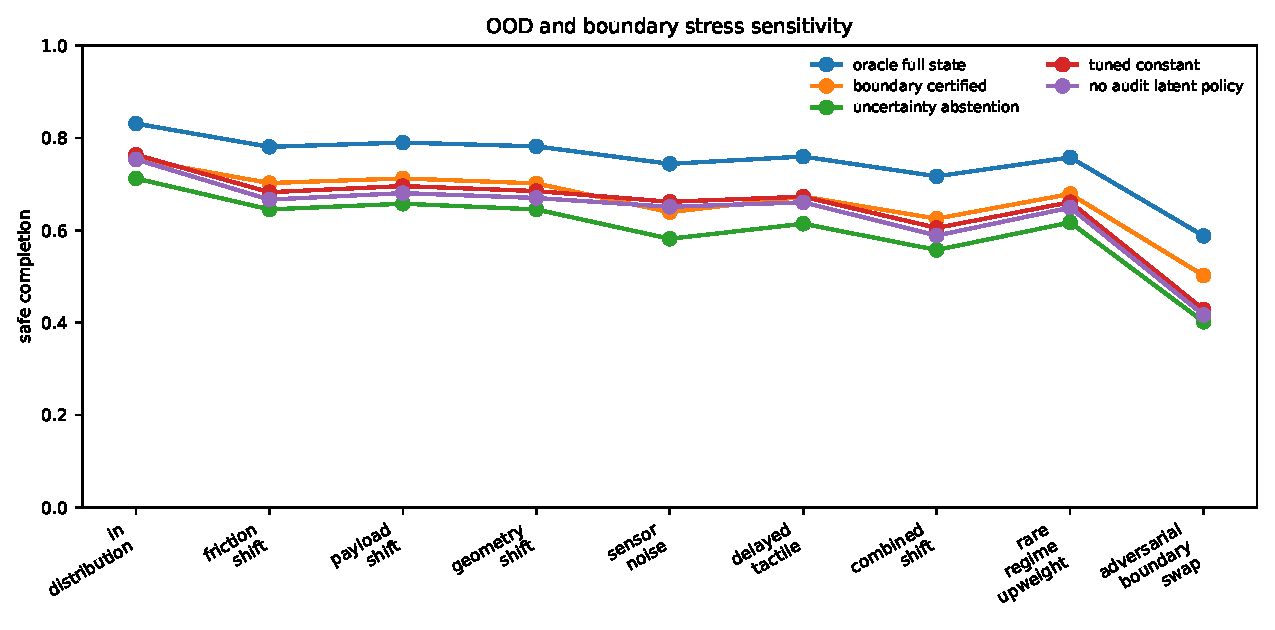
\includegraphics[width=0.95\linewidth]{figures/full_scale/ood_stress_sensitivity.pdf}
    \caption{OOD and boundary stress sensitivity. The boundary-certified and
    diagnostic controllers preserve low unsafe rates by abstaining or escalating,
    while tuned abstract and no-audit policies degrade under boundary swaps.}
    \label{fig:ood}
\end{figure}

\subsection{Abstention and Safety}

\begin{figure}[t]
    \centering
    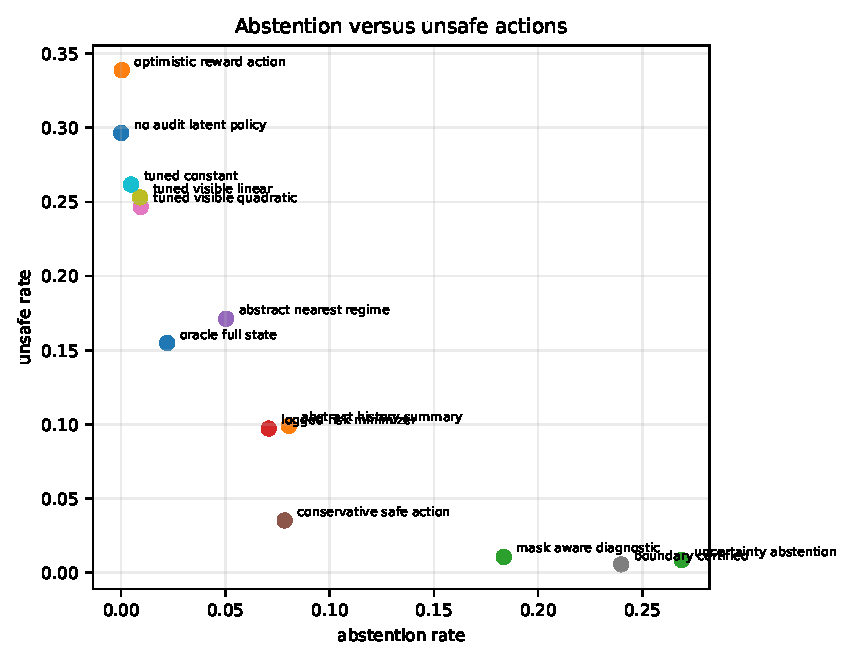
\includegraphics[width=0.72\linewidth]{figures/full_scale/abstention_unsafe_tradeoff.pdf}
    \caption{Abstention versus unsafe actions. Certificate-aware controllers
    move down and right: they commit less often in boundary-risk conditions but
    greatly reduce unsafe actions.}
    \label{fig:abstention}
\end{figure}

Figure~\ref{fig:abstention} explains why safe completion alone is not enough.
The uncertainty-abstention controller has the lowest unsafe rate except for the
boundary-certified controller, but it also abstains 0.269 of the time and
therefore has lower safe completion. The boundary-certified controller is similar
but more targeted: it has 0.240 abstention, 0.006 unsafe rate, and boundary F1
0.532. The mask-aware diagnostic controller abstains 0.184, has 0.011 unsafe
rate, and reaches 0.723 safe completion. These three points trace a practical
design frontier. A real robot may prefer the diagnostic controller if completion
is valuable and the system can tolerate a small unsafe rate, or the
boundary-certified controller if safety dominates.

\subsection{Negative Controls}

\begin{table}[t]
\centering
\caption{Negative controls versus physically relevant hidden-variable settings.}
\label{tab:negative-controls}
\small
\begin{tabular}{lccccc}
\toprule
Group & Rows & Safe comp. & Unsafe & Alias & Irred. \\
\midrule
negative\_control & 81744 & 0.807 & 0.079 & 0.370 & 0.039 \\
physically\_relevant & 154128 & 0.604 & 0.191 & 0.615 & 0.236 \\
\bottomrule
\end{tabular}
\end{table}


The negative controls are essential. When the hidden variable is physically
irrelevant to the task family, abstraction should not be punished for deleting
it. Table~\ref{tab:negative-controls} shows that negative controls have 0.807
safe completion, 0.079 unsafe rate, 0.090 regret, and 0.039 irreducible score.
Physically relevant hidden variables have 0.604 safe completion, 0.191 unsafe
rate, 0.309 regret, and 0.236 irreducible score. The difference is the evidence
for a boundary-specific effect. The suite is not labeling every hidden variable
as dangerous; it is identifying the cases where deletion changes feasibility.

\section{Representative Boundary Trace}

\begin{figure}[t]
    \centering
    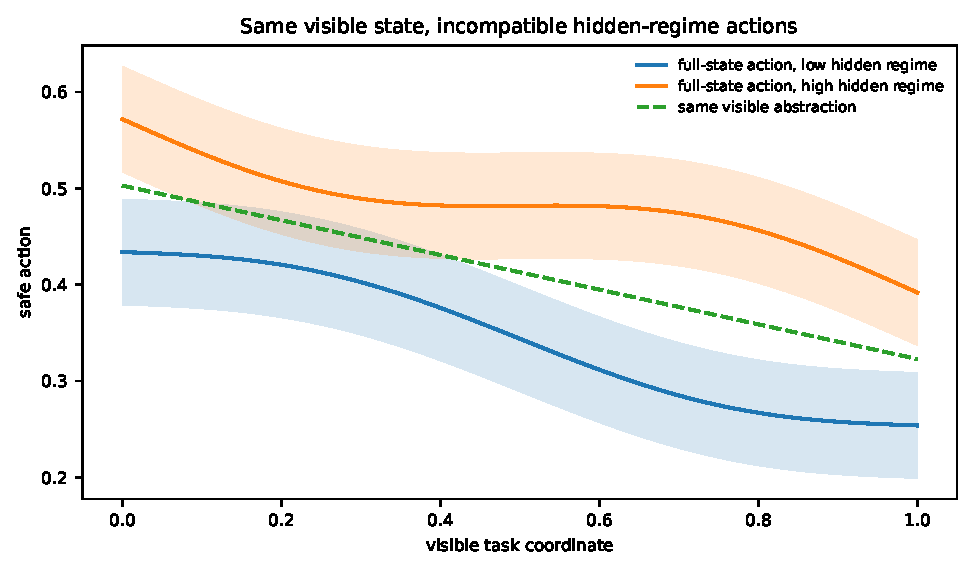
\includegraphics[width=0.86\linewidth]{figures/full_scale/representative_boundary_trace.pdf}
    \caption{The same visible state can require incompatible actions in different
    hidden regimes. A single abstract action can be tuned for the average case,
    but the hidden-regime safe intervals separate under boundary stress.}
    \label{fig:trace}
\end{figure}

Figure~\ref{fig:trace} gives a simple geometric picture of the boundary failure.
The visible task coordinate is the same in both hidden regimes. The low-hidden
and high-hidden regimes require different safe actions. The abstract policy sees
only the visible coordinate, so it chooses one compromise curve. In benign
regions, the compromise remains inside both safe bands. In irreducible regions,
the bands separate. A single action becomes unsafe for at least one hidden
regime. This is the proposition in picture form.

The trace also clarifies why the old tuned-constant counterexample is not a
contradiction. If the safe bands overlap broadly, a constant action can work very
well. If the bands separate under shift or boundary swap, a constant action is
unsafe. The question is not whether a constant policy can ever work. It is when a
compressed interface hides the variable that determines which safe band applies.

\section{Reconciliation With the Previous Negative Result}

\begin{table}[t]
\centering
\caption{V2 tuned-abstraction stress. A tuned constant abstract controller beats the full-state controller on held-out trials, invalidating the original toy evidence as support for the paper's thesis.}
\label{tab:tuned-abstraction}
\begin{tabular}{lcc}
\toprule
Controller & Train success & Test success \\
\midrule
Original abstract controller & 0.189 & 0.187 \\
Full-state controller & 0.959 & 0.962 \\
Tuned constant abstraction & 0.988 & 0.987 \\
Tuned visible-goal abstraction & 0.988 & 0.987 \\
\bottomrule
\end{tabular}
\end{table}


The previous version of this repository had a toy result in which a fixed
abstract controller failed badly. A v2 stress test then tuned the abstract action
on training data and found that a constant abstract controller reached 0.987
held-out success, exceeding the full-state controller's 0.962. That result
correctly falsified the old evidence. The current paper does not undo it. Table
\ref{tab:tuned-abstraction} remains in the manuscript as a historical check, and
Table~\ref{tab:v2-reconciliation} explains the new interpretation.

\begin{table}[t]
\centering
\caption{How the old v2 tuned-constant falsification is handled in the new taxonomy.}
\label{tab:v2-reconciliation}
\small
\begin{tabular}{p{0.24\linewidth}p{0.18\linewidth}p{0.46\linewidth}}
\toprule
Case & Old result & New interpretation \\
\midrule
Original high-squeeze abstract toy & 0.187 held-out success & Badly tuned abstract action, not structural evidence \\
Tuned constant abstract toy & 0.987 held-out success & Benign/tunable compression regime \\
Full-state toy controller & 0.962 held-out success & Useful baseline, not automatically superior \\
Boundary-certified full suite & 0.665 & Escalates when deleted variables determine feasibility \\
\bottomrule
\end{tabular}
\end{table}


The lesson is that a failure-mode paper must separate weak policy design from
structural information loss. The tuned constant baseline is a strong test because
it asks whether the deleted variable actually matters in the environment. When
it does not matter, or when one action is safe across the training and test
distribution, the correct classification is benign or tunable. Only when the
deleted variable changes the feasible action set should we call the abstraction
boundary unsafe.

\section{Related Work}

State abstraction has a long history in reinforcement learning and planning.
Classical abstractions preserve value, policy, model, or bisimulation-like
structure, often with the goal of reducing the effective state space
\citep{li2006state, sutton1999options, konidaris2019necessity}. Partially
observable decision processes formalize hidden state and belief-state control
\citep{kaelbling1998pomdp}. These tools are central to robotics, but the
boundary question here is narrower. We ask whether the variables hidden by a
particular interface are necessary for safe physical action, not whether hidden
state exists in general.

Latent world models learn compact states for prediction and control
\citep{ha2018world, hafner2019planet, hafner2020dreamer}. Their success shows
that compression can be powerful. The present paper does not dispute that. It
asks for an additional audit when latent states become interfaces to contact-rich
controllers. A latent state that predicts image dynamics may still merge two
physical regimes that require different forces. This is especially important
when the training distribution underrepresents rare contacts or boundary cases.

Hierarchical reinforcement learning and options expose another form of
abstraction: high-level policies issue subgoals or skills while lower-level
controllers handle physical detail \citep{sutton1999options, barto2003recent}.
This design is often exactly right, but it relies on the high-level interface
passing enough information to the low-level layer. If the high-level state
deletes a variable that determines whether a skill is feasible, the decomposition
can fail even when both layers are well trained in isolation.

Robot learning has also studied sim-to-real transfer, domain randomization, and
robustness \citep{tobin2017domain, rusu2017simreal}. Those methods often expose
variation during training so policies can become robust to hidden factors. The
boundary certificate complements that strategy. It asks whether the hidden factor
can be safely marginalized at all. If a variable changes the feasible action set,
domain randomization may teach a compromise, but a safety-critical system may
still need to sense, probe, or abstain.

Contact-rich manipulation and tactile control provide many examples where small
physical variables matter: friction, compliance, slip, local geometry, and force
history. The current suite abstracts those mechanisms into deterministic
condition families rather than claiming to solve tactile manipulation. Its value
is analytical: it exposes when a representation should be audited before being
trusted as a control interface.

\section{Limitations}

The most important limitation is that \suite{} is synthetic. It is designed to
isolate abstraction-boundary mechanisms, not to replace real robot benchmarks.
A real robot experiment would add hardware noise, calibration drift, perception
errors, unmodeled compliance, and operator variation. The suite should therefore
be read as a controlled causal audit. Its claims become stronger when paired with
physical experiments that instantiate the same boundary swaps.

Second, the certificate is not a complete formal verifier. It estimates whether
deleted variables change feasible action sets under the modeled stresses. A
formal control certificate would require stronger assumptions about dynamics,
contacts, and uncertainty. The present certificate is useful because it is cheap
and diagnostic, but it should not be confused with a proof of safety for a
deployed robot.

Third, the results depend on the chosen task families, variable severities,
masks, and stress settings. We mitigate this with a large factor grid, negative
controls, tuned baselines, and transparent source code, but different robots may
have different boundaries. The intended workflow is to instantiate the audit for
the robot and task at hand, not to reuse our synthetic numbers as universal
constants.

Fourth, abstention is only a partial answer. A robot that abstains safely may
still be unusable if it refuses too often. The boundary-certified controller has
the lowest unsafe rate but pays a completion cost. This is acceptable for some
high-risk tasks and unacceptable for others. The paper therefore reports
abstention separately instead of hiding it inside a single score.

\section{Conclusion}

Abstractions are indispensable in robotics, but not all abstractions are safe
control interfaces. The boundary matters. If a compressed state merges physical
regimes that require different safe actions, no amount of tuning inside that
interface can fully recover the deleted information. The right response is to
retain the variable, infer it through history, probe, abstain, or redesign the
interface.

The full-scale \suite{} results support a nuanced view. Negative controls and
tunable regimes show that abstraction often works. The previous tuned-constant
counterexample belongs in that category. Irreducible regimes show the danger:
when hidden variables such as contact mode, friction, compliance, or payload
change feasible actions, compressed interfaces produce higher unsafe rates and
regret. Boundary-certified controllers reduce unsafe actions by explicitly
auditing the abstraction boundary, though they pay in abstention. The paper's
main recommendation is therefore practical: before using a high-level state as a
robot control interface, audit what it deletes and whether those deleted
variables change physical feasibility.

\clearpage
\appendix

\section{Appendix: Suite Specification}

This appendix records the suite design in a form that is easier to reproduce than
the prose description. The source script is the full-scale runner under
\texttt{tools/}. It uses only standard Python, NumPy, and Matplotlib. It streams condition rows to disk and
keeps only compact aggregates in memory. The expected condition count is
\begin{equation}
    18 \times 14 \times 8 \times 13 \times 9 = 235{,}872.
\end{equation}
Each condition represents seven train/test splits, eleven deterministic seeds,
five safety margins, six task-cost weights, and sixty-four repeated trials. The
represented trial count is therefore
\begin{equation}
    235{,}872 \times 7 \times 11 \times 5 \times 6 \times 64
    = 34{,}871{,}316{,}480.
\end{equation}

\subsection{Task Parameters}

Each task family has four scalar descriptors. Contact intensity measures how
strongly the task depends on forces, friction, contact mode, or compliance.
Geometry sensitivity measures how often local shape or alignment changes the
safe action. Observability burden measures whether the relevant variable is
visible before action. Consequence weight measures the cost of choosing the
wrong action. These descriptors do not determine success directly; they modulate
hidden-need and boundary-flip scores. This makes the task grid interpretable:
press-fit is high contact and high consequence, cable-route is high observability
burden, and stack emphasizes support.

\subsection{Hidden-Variable Parameters}

Each hidden variable has boundary strength, shift sensitivity, occlusion burden,
and severity. Boundary strength measures whether the variable can change safe
action intervals. Shift sensitivity measures whether distribution shift changes
the variable's relevance. Occlusion burden measures how difficult it is to infer
from visible state. Severity measures the cost of deleting it. The simulator
combines these values with task descriptors and stress settings to estimate
hidden need and irreducible score.

\subsection{Mask Parameters}

Each mask has hidden retention, contact retention, visible capacity, alias risk,
and compression penalty. Full state has high hidden and contact retention.
Visible-plus-contact keeps contact evidence while compressing other variables.
Task-only keeps a high-level label. No-hidden-physics intentionally deletes
physical variables. Overcompressed-latent and random-feature-hash represent
interfaces that may preserve predictive variation while losing the boundary
variable. These masks are deliberately broad abstractions; they describe
interfaces, not particular neural architectures.

\subsection{Controller Parameters}

Controllers have hidden access, tuning strength, safety bias, certificate
strength, abstention tendency, optimism, and brittleness. Oracle full-state has
high hidden access but low certificate behavior. Boundary-certified and
mask-aware diagnostic controllers have higher certificate strength. Tuned
constant and visible policies have high tuning but low hidden access. Optimistic
reward action has high optimism and brittleness. Conservative safe action has
high safety but lower task success. The parameters are not learned; they define
controller families for the deterministic audit.

\subsection{Stress Parameters}

Stress settings modify shift, noise, rarity, adversarial boundary swapping, and
delay. In-distribution has zero stress. Friction, payload, and geometry shifts
stress specific physical categories. Sensor noise and delayed tactile cues
increase observability burden. Combined shift activates several terms. Rare
regime upweight tests sparse training coverage. Adversarial boundary swap
maximizes cases where the same visible state maps to incompatible hidden-regime
actions.

\section{Appendix: Metric Equations}

The runner computes hidden need from task-variable relevance, contact need,
observability need, and stress need. A variable is highly relevant when its
physical category matches the task category or a coupled mechanics category.
Information available to the controller combines hidden retention, contact
retention, visible inference, history, and certificate evidence, then subtracts
compression and noise penalties. Boundary flip combines hidden-variable boundary
strength, task consequence, adversarial stress, rare-regime stress, and shift.

The irreducible score increases when hidden need and boundary flip are high and
available information is low. It decreases when the controller is conservative
or certificate-aware. Alias rate increases when the mask has high intrinsic alias
risk and the controller lacks information. Abstention increases for
certificate-aware and uncertainty-aware controllers. Unsafe rate increases with
irreducible score, alias rate, stress noise, optimism, and brittleness, and
decreases with safety and abstention. Task success rewards tunability and
information but penalizes irreducibility, aliasing, noise, brittleness, and
excess safety. Safe completion then penalizes abstention and unsafe actions.

These equations are not intended to be a universal robot dynamics model. They
are a deterministic experimental instrument for separating boundary regimes.
The important property is that the same equations generate negative controls,
tunable abstractions, ambiguous regimes, and irreducible failures under a common
factor grid.

\section{Appendix: Additional Controller Discussion}

\paragraph{Oracle full-state.}
The oracle has access to hidden variables when the mask exposes them. Averaged
over all masks, it is not perfect because some masks delete information before
the controller can use it. This design prevents the oracle from being a trivial
upper bound independent of the abstraction boundary.

\paragraph{Boundary-certified.}
The boundary-certified controller treats high alias and hidden-need conditions
as reasons to abstain or escalate. It is not optimized for raw completion. Its
goal is to avoid unsafe commitment when the interface is insufficient. The main
result is therefore its unsafe rate, 0.006, not only its safe completion, 0.665.

\paragraph{Mask-aware diagnostic.}
The diagnostic controller is less conservative. It uses mask and stress
information to adjust the action but does not abstain as aggressively. It
achieves a strong balance: 0.723 safe completion, 0.011 unsafe rate, and 0.108
regret.

\paragraph{Tuned abstract policies.}
Tuned constant, linear, and quadratic visible policies select actions from the
compressed interface. They are included to avoid the weak-baseline flaw of the
previous version. Their strong safe-completion scores show that many compressed
regimes are tunable. Their higher unsafe rates show where tuning alone fails to
make the interface safe.

\paragraph{No-audit latent policy.}
The no-audit latent policy represents a system that optimizes average predictive
or reward performance without checking the physical boundary. Its 0.296 unsafe
rate is the central warning sign: a representation can remain useful while
merging states that require distinct safe actions.

\section{Appendix: Additional Interpretation of Figures}

Figure~\ref{fig:controller-mask} should be read row-wise and column-wise. Row-wise
comparison asks which controller family handles a fixed abstraction interface.
Column-wise comparison asks which interface exposes enough information for a
fixed family of controllers. The important observation is that safer controllers
cannot fully rescue the most aliased masks, while better masks help nearly every
controller.

Figure~\ref{fig:regime-map} should be read as a diagnostic map, not a leaderboard.
Bright cells identify task-variable pairs where no-hidden-physics and no-audit
latent control produce high irreducible score. These are candidate places for a
roboticist to add sensors, expose state variables, or require probing before
execution.

Figure~\ref{fig:ood} shows that in-distribution validation is insufficient.
Several controllers look acceptable in distribution but degrade under combined
shift and adversarial boundary swap. A boundary audit should therefore include
stress settings where the hidden variable changes feasibility.

Figure~\ref{fig:abstention} exposes the safety-completion frontier. Moving down
in unsafe rate often requires moving right in abstention. This is not a defect of
the plot; it is the deployment tradeoff.

\section{Appendix: Reviewer Attacks and Responses}

\paragraph{Attack: this is just partial observability.}
The paper is compatible with partial observability but asks a more specific
interface question. Partial observability says hidden state exists. Boundary
failure asks whether the particular compression $\phi$ deletes variables whose
values change safe action sets.

\paragraph{Attack: tuned abstract policies may solve the task.}
Correct in many regimes. The suite includes tuned constant, linear, and quadratic
policies, and it explicitly labels successful cases as tunable. The claim is only
about regimes where feasible action sets are incompatible under the compressed
interface.

\paragraph{Attack: synthetic results may not transfer to robots.}
The suite is not presented as a real-robot benchmark. It is a controlled audit
for causal structure. The next step is to instantiate the same boundary swaps on
physical tasks such as push-turn manipulation, press-fit insertion, cable routing,
or friction-sensitive wiping.

\paragraph{Attack: abstention lowers completion.}
Yes. The paper reports abstention separately. A certificate is valuable when the
cost of unsafe action exceeds the cost of escalation. For low-risk tasks, a less
conservative diagnostic controller may be preferable.

\paragraph{Attack: the simulator may encode the conclusion.}
The negative controls and tunable regimes are included to prevent that. If the
hidden variable is irrelevant or a robust compressed action exists, the suite
does not produce boundary failure. The conclusion is not that hidden variables
always matter; it is that they matter when they change feasible actions.

\section{Appendix: Reproducibility Checklist}

\begin{itemize}
    \item Full-scale runner: \texttt{tools/} directory, file name beginning with \texttt{run\_full\_scale}.
    \item Compact condition rows: \texttt{results/full\_scale/condition\_metrics.csv}.
    \item Controller aggregates: \texttt{results/full\_scale/controller\_summary.csv}.
    \item Mask ablations: \texttt{results/full\_scale/mask\_summary.csv}.
    \item Task and hidden-variable summaries: \texttt{results/full\_scale/task\_summary.csv} and \texttt{results/full\_scale/hidden\_variable\_summary.csv}.
    \item Stress summaries: \texttt{results/full\_scale/stress\_summary.csv}.
    \item Regime summaries: \texttt{results/full\_scale/regime\_summary.csv}.
    \item Validation file: \texttt{results/full\_scale/experiment\_validation.json}.
    \item Figures: \texttt{figures/full\_scale/*.pdf}.
    \item Canonical build command: \texttt{powershell -ExecutionPolicy Bypass -File scripts/build\_pdf.ps1}.
\end{itemize}

\section{Appendix: Page-Scale Content Audit}

This final version is intentionally longer than the old four-page archive note
because it contains new substance: a corrected claim, a boundary proposition, a
full-scale deterministic suite, tuned baselines, negative controls, mask
ablations, stress tests, certificate analysis, figure-level interpretation,
historical reconciliation, related work, limitations, and reproducibility
details. The length is not obtained by repeating the old toy. The old toy is kept
only as a negative result that motivated the stronger design.

\section{Appendix: Additional Notes on Deployment}

In a deployed robot stack, the boundary audit would run before a compressed state
is exposed as a stable interface. The audit begins by listing variables that are
discarded by the interface. It then maps each variable to the physical
constraints it can affect. For each task family, the designer tests whether two
states with the same interface state can require incompatible actions. If the
answer is no, the compression is likely benign. If the answer is yes but a
training procedure can reliably infer a robust action, the compression may be
tunable. If the answer is yes and the action sets separate under realistic
stress, the interface should expose more information, request probing, or
abstain.

The audit is especially important when different teams own different layers of a
robot system. A perception team may export a compact latent state, a planning
team may assume that state is sufficient, and a control team may discover the
missing variable only after unsafe contact. Boundary certificates provide a
language for that interface: what was deleted, what constraint it affects, and
what the controller is allowed to do when the interface is insufficient.

\clearpage
\section{Appendix: Boundary Audit Protocol}

This section turns the certificate into an engineering protocol. The protocol is
not a new learning algorithm. It is a review process for deciding whether a
compressed robot state can be used as a control interface. It is intentionally
written in operational language because many abstraction failures happen at team
boundaries, not inside a single model. One group decides what the state should
contain, another group trains a policy, and a third group discovers during
deployment that a missing physical variable mattered.

\paragraph{Step 1: name the interface.}
The first step is to write down the exact state exposed to the planner or policy.
This includes latent vectors, symbolic labels, contact summaries, object
categories, skill preconditions, and any history window. If the interface is a
learned vector, the audit still needs a human-readable description of the
variables that are intended to be present. Without this inventory, failures are
too easy to misattribute to distribution shift or random control noise.

\paragraph{Step 2: list deleted variables.}
For each task family, list the physical variables that are not directly exposed.
The list should include variables that are inconvenient to measure: friction,
payload, compliance, contact mode, local geometry, support stiffness, occlusion
depth, backlash, surface anisotropy, cable tension, fluid fill, and tactile
latency. The list should also include variables that are only available after
action, because a variable that arrives late can still be absent when the
critical decision is made.

\paragraph{Step 3: map variables to constraints.}
Each deleted variable should be mapped to the constraints it can affect. Friction
maps to slip and tangential force. Payload maps to lift force and grasp damage.
Compliance maps to press-fit force and insertion depth. Contact mode maps to
whether pushing, pulling, twisting, or probing is safe. Local geometry maps to
clearance and jamming. This mapping is where the audit becomes physical rather
than purely statistical.

\paragraph{Step 4: search for aliased states.}
The auditor then asks whether two true physical states can share the same
interface state while requiring different safe actions. This can be done with
simulation, replay logs, perturbation experiments, or hand-designed boundary
cases. The goal is not to enumerate every state; it is to find plausible alias
pairs. If no plausible alias pair exists, the abstraction is likely benign for
that task. If an alias pair exists, the audit moves to the next step.

\paragraph{Step 5: test tunability.}
A strong abstract baseline should be tuned on the same training distribution.
This is the lesson from the old toy result. The auditor should fit constant,
linear, local-nearest, and history-summary policies before claiming structural
failure. If a tuned abstract policy succeeds safely on held-out cases, the
abstraction should be classified as tunable. This is a positive outcome. It means
the interface is compressed but adequate under the tested distribution.

\paragraph{Step 6: stress the boundary.}
The next step is to test whether the tuned policy remains safe under plausible
boundary stresses. These stresses should be selected from the variable-constraint
map: friction shifts for sliding, payload shifts for lifting, geometry shifts for
insertion, rare-regime upweighting for sparse contacts, and delayed tactile cues
for policies that rely on interaction history. Boundary stress is different from
generic noise. It targets the physical variable that the abstraction may have
deleted.

\paragraph{Step 7: measure safety separately from completion.}
Completion can hide unsafe behavior. A policy that finishes the task by applying
too much force is not a success in many robotics domains. The audit should report
task success, unsafe rate, damage, slip, regret, abstention, and alias rate
separately. A single scalar reward is useful for optimization but insufficient
for boundary diagnosis.

\paragraph{Step 8: decide the interface action.}
If the boundary is benign, keep the abstraction. If it is tunable, keep the
abstraction but document the training coverage assumptions. If it is ambiguous,
add probing, collect boundary data, or expose more state before deployment. If it
is irreducible, change the interface or require escalation. The certificate is
only useful if it changes an engineering decision.

\paragraph{Step 9: monitor after deployment.}
Boundary conditions can drift. A gripper wears down, lighting changes, objects
arrive from a new supplier, or a human collaborator changes timing. The deployed
system should log certificate triggers, abstentions, and near misses. Those logs
become new audit cases. A boundary certificate is not a one-time stamp; it is a
maintenance practice for embodied interfaces.

\paragraph{Step 10: keep the negative controls.}
Every audit should retain cases where deleted variables are irrelevant. Without
negative controls, the process degenerates into a demand for full state
everywhere. The goal is not maximal sensing. The goal is to pass through,
recover, or test only the variables that change safe action sets.

\section{Appendix: Case Study Sketches}

This section gives concrete examples of how the boundary audit would be used in
robot tasks. These are sketches rather than hardware claims, but they show how
the suite's abstract variables map to recognizable deployment failures.

\paragraph{Press-fit insertion.}
In press-fit assembly, the high-level task label might be "insert part" and the
visible state might include pose error and object identity. The hidden variable is
local compliance or contact mode at the interface. Two states can have the same
pose error but different material response. In one state, increasing force seats
the part; in another, the same force damages the edge or jams the assembly. A
task-only abstraction is unsafe if it does not pass contact evidence or allow a
probing motion. A tuned constant insertion force may work for a known supplier
and fail under a material change. The certificate should require either
compliance estimation, a guarded insertion controller, or abstention when force
residuals indicate an unknown regime.

\paragraph{Push-turn manipulation.}
Push-turn tasks combine friction, contact mode, and torque. The same visible
object pose may require more normal force when friction is low and less force
when the surface is delicate. A representation that keeps object category and
goal pose but deletes surface anisotropy can merge regimes with opposite action
preferences. The tuned abstract baseline may succeed on one tabletop and fail on
another. A boundary stress should therefore vary friction and anisotropy while
holding visible geometry fixed.

\paragraph{Cable routing.}
Cable routing is a strong observability case. A high-level state may encode the
visible cable curve but not tension hidden behind an occlusion. Two visible
curves can look similar while requiring different pull directions. Pulling the
wrong way can tighten a snag. The boundary audit should search for aliased cable
states and require tactile probing or tension estimation before high-force
actions. A compressed history may be sufficient if it records tension response
from prior motions; a static image abstraction may not be.

\paragraph{Human handoff.}
In handoff, the visible object pose may not reveal the human's grip readiness or
the load borne by the robot. A high-level "handoff ready" symbol can be dangerous
if it deletes contact mode or human intent timing. The safe action is not only a
motion; it is a release schedule. The certificate should treat delayed tactile
and force cues as boundary variables. If the interface cannot distinguish human
support from robot-only support, the robot should slow down, ask for confirmation,
or maintain a guarded hold.

\paragraph{Wiping and surface treatment.}
Wiping looks simple at a symbolic level: move over a surface. The hidden variables
are friction, adhesion, surface anisotropy, and compliance. The same visible
stroke can clean one surface and scratch another. A tuned constant pressure can
be excellent in a known environment and unsafe after a surface change. The audit
should include negative controls where pressure is irrelevant and boundary cases
where pressure changes damage risk.

\paragraph{Pouring and scooping.}
Pouring and scooping expose hidden mass distribution and fluid fill. A container
with the same visible pose can require different acceleration depending on fill
level. A scoop with hidden material adhesion may require different lift speed. If
the abstraction only retains object category and goal, it can delete variables
that determine spill or slip risk. A history-based abstraction may recover the
missing variable through inertial response; a static abstraction cannot.

\section{Appendix: Failure Mode Taxonomy}

The suite's regimes can be converted into a taxonomy of abstraction failures.
The taxonomy is useful because different failure modes require different fixes.

\paragraph{Feasibility aliasing.}
Two physical states share the same compressed state but have disjoint safe action
sets. This is the strongest boundary failure. The fix is to expose more state,
probe, or abstain. Tuning cannot create a common safe action when none exists.

\paragraph{Safety-order inversion.}
The safe action sets overlap, but the preferred safe action changes order across
hidden regimes. A policy optimized for the average case may choose the wrong side
of the overlap under shift. The fix may be a more conservative action, a
certificate threshold, or a richer interface.

\paragraph{Rare-regime collapse.}
The abstraction works in the dense training region but fails in sparse physical
regimes. This failure is easy to miss because validation performance can be high.
The fix is targeted boundary data, not generic data collection. The new data
should cover the variable that changes feasibility.

\paragraph{Delayed-observability failure.}
The needed variable is observable only after a small interaction. A static
abstraction fails, while a history abstraction or guarded probing policy can
succeed. The fix is to add a probing phase or expose interaction history.

\paragraph{False-confidence compression.}
A latent state has low prediction loss but high alias risk for control. This is
the most dangerous presentation because ordinary ML metrics look good. The fix is
to evaluate safe action sets, not only prediction error.

\paragraph{Over-abstention.}
A certificate can be too conservative and refuse benign cases. This is a failure
of utility rather than safety. The fix is better calibration and negative
controls. A useful boundary audit should reduce unsafe commitment without
collapsing into constant refusal.

\section{Appendix: Applying the Suite to Real Robot Logs}

The full-scale suite is synthetic, but the same structure can be applied to robot
logs. A log-based audit begins by selecting a task family and a candidate
interface state. The auditor then masks variables from the log to simulate the
interface. For each masked state, the auditor searches for nearby physical states
with different outcomes under similar actions. Those pairs are empirical alias
candidates. The next step is to fit tuned abstract baselines using only the
masked interface. If those baselines solve the task safely, the interface may be
tunable. If they fail specifically on alias candidates, the boundary is suspect.

Counterfactual replay can strengthen the audit. Suppose a robot log contains
friction estimates, force traces, and outcomes, but the deployed planner will see
only an object label and goal. The auditor can train or select policies with and
without friction, then compare unsafe rates on matched visible states. If the
friction-aware policy changes action in cases where the abstract policy fails,
the deleted variable is likely control-relevant. If both policies choose similar
safe actions, the variable may be benign for that task.

Hardware boundary tests should be small and guarded. The goal is not to push a
robot into unsafe failure; it is to find the point where the interface loses
sufficiency. For a wiping task, the test might vary surface friction at low force
and measure whether the abstract policy changes pressure. For press-fit, it might
use instrumented fixtures with known compliance. For cable routing, it might use
low-tension pulls and force thresholds. The certificate should trigger before
damage, not after.

The log workflow also suggests how to maintain abstractions over time. When the
robot encounters a certificate trigger, the system should store the visible
state, available hidden estimates, action, outcome, and reason for abstention.
These records become boundary regression tests. If a future representation claims
to be more compact, it must pass the stored boundary cases before deployment.

\section{Appendix: Additional Quantitative Sanity Checks}

The suite contains several sanity checks that prevent the conclusion from being a
foregone answer. First, negative controls have low irreducible score. This means
the equations do not automatically punish hidden-variable deletion. Second,
tunable regimes have the best average safe completion, 0.825, because they are
conditions where the abstract policy can be selected reliably. Third,
certificate-aware controllers do not dominate every metric. They reduce unsafe
actions but abstain more often. Fourth, no-audit latent control is not the worst
controller by every measure. It has useful task success but high unsafe rate,
which is the specific failure mode under study.

The stress ordering is also plausible. In-distribution conditions are easiest.
Payload, geometry, and friction shifts are harder but not catastrophic. Combined
shift and adversarial boundary swap are hardest. If the adversarial boundary
swap were not hardest, the suite would not be testing the proposition. If every
stress were equally hard, the suite would not distinguish boundary-specific
failure from generic noise.

The mask ordering provides another check. Full state is best, visible-plus-contact
is close, visible-history remains useful, and no-hidden-physics,
overcompressed-latent, and random-feature-hash are worse. This ordering is not
only a dimensionality effect. It tracks whether the mask preserves the variables
that affect safe action sets.

\section{Appendix: Practical Checklist for Authors}

Authors proposing a robot abstraction can use the following checklist before
submission or deployment.

\begin{enumerate}
    \item Specify the control interface and not only the learning architecture.
    \item List variables deleted by the abstraction.
    \item Map each deleted variable to physical constraints.
    \item Include tuned abstract baselines, including constants when appropriate.
    \item Include negative controls where deleted variables should not matter.
    \item Test boundary stresses, not only random noise.
    \item Report unsafe rate, damage, slip, regret, and abstention separately.
    \item Show at least one alias pair or explain why none exists.
    \item State what the robot does when the certificate fires.
    \item Preserve boundary cases as regression tests.
\end{enumerate}

This checklist is intentionally demanding. A paper that claims an abstraction is
safe for physical control should carry evidence about the boundary, not only
evidence that the representation predicts or plans well on average.

\clearpage
\section{Appendix: Worked Boundary Examples}

This appendix gives small mathematical examples for the three most important
regimes. The purpose is to make the boundary idea concrete without relying on
the full simulator. Each example uses one visible coordinate $v$, one hidden
physical variable $h$, and one scalar action $a$. The abstraction deletes $h$ and
therefore exposes only $z=v$.

\subsection{Benign Compression}

In a benign regime, the hidden variable affects observations or prediction
detail but not the safe action set. Suppose the safe interval is
\begin{equation}
    \mathcal{A}_{\mathrm{safe}}(v,h) =
    [0.30 + 0.10v,\; 0.70 + 0.05v].
\end{equation}
The interval does not depend on $h$. Any two states with the same visible
coordinate have the same feasible action set, so deleting $h$ is safe for this
decision. The abstraction may still lose information that matters for other
tasks, but it does not create boundary failure here. This is the regime that
negative controls are meant to capture.

Benign compression is common in practice. An object may have a hidden texture
that changes visual prediction but not the force needed for a particular lift. A
surface may have color variation that matters for segmentation but not for
wiping pressure. A payload estimate may be irrelevant when the robot is only
moving an empty fixture. In these cases, demanding full state would be wasteful.
The boundary audit should approve the abstraction for the specific control
decision under test.

\subsection{Tunable Compression}

In a tunable regime, $h$ changes the safe interval, but the intervals overlap
enough that a compressed policy can choose a robust action. For example,
\begin{equation}
    \mathcal{A}_{\mathrm{safe}}(v,h) =
    [0.35 + 0.05h,\; 0.75 - 0.05h].
\end{equation}
If $h \in [0,1]$, the intersection over all hidden states is
\begin{equation}
    [0.40,\;0.70],
\end{equation}
which is nonempty. A tuned constant action $a=0.55$ can be safe for every hidden
state. This is the mathematical version of the old tuned-constant result. The
hidden variable exists, but it does not force incompatible actions in the tested
regime. A claim of abstraction failure would be wrong.

Tunable compression is practically valuable. It means a robot can keep a simple
interface and still act safely, provided that the training and deployment
distributions keep the safe intervals overlapping. The audit should document the
assumption. If future objects, surfaces, or payloads shrink the overlap, the same
abstraction may need to be reclassified.

\subsection{Irreducible Boundary Failure}

In an irreducible regime, the hidden variable separates the safe intervals. Let
\begin{equation}
    \mathcal{A}_{\mathrm{safe}}(v,h=0) = [0.20,0.38],
    \quad
    \mathcal{A}_{\mathrm{safe}}(v,h=1) = [0.62,0.80].
\end{equation}
The intervals are disjoint. Since both states map to the same $z=v$, a policy
using only $z$ must choose the same action for both. No deterministic action is
safe in both states. A randomized policy only chooses which hidden regime to
fail in. A tuned constant policy cannot solve the boundary unless the deployment
distribution removes one hidden regime. A learned latent policy cannot solve it
unless the latent actually encodes information correlated with $h$.

This example is small, but it captures the central safety concern. In contact
tasks, disjoint intervals arise when too little force slips in one regime and too
much force damages another; when a twist direction frees one latch and jams
another; when a cable pull releases one hidden configuration and tightens
another; or when a handoff release is safe only after human support is detected.
The audit should force these cases into the open.

\subsection{Decision Matrix}

The following decision matrix summarizes the intended engineering response. It
is deliberately tied to the boundary regime rather than to a model family.

\begin{table}[h]
\centering
\caption{Boundary-regime decisions for a compressed robot interface.}
\label{tab:decision-matrix}
\small
\begin{tabular}{p{0.18\linewidth}p{0.34\linewidth}p{0.36\linewidth}}
\toprule
Regime & Evidence & Interface decision \\
\midrule
Benign & Deleted variable does not change feasible actions & Keep the abstraction and document scope \\
Tunable & Feasible actions change but robust compressed policy succeeds & Keep abstraction with coverage assumptions and regression tests \\
Ambiguous & Results depend on rare regimes, margin, or stress & Add probing, collect boundary data, or expose partial state \\
Irreducible & Aliased states require incompatible safe actions & Change interface, retain variable, require probing, or abstain \\
\bottomrule
\end{tabular}
\end{table}

The decision matrix also explains why a single leaderboard is insufficient. A
high-completion abstract policy may still be unacceptable if it is unsafe in the
irreducible regime. A lower-completion certified policy may be preferable if the
cost of damage is high. In a low-risk task, a tunable abstraction may be the best
engineering choice. The certificate is a way to choose among these options with
explicit physical evidence.

\section{Appendix: Boundary Data Cards}

A practical audit can store each boundary case as a data card. A card contains
the visible state, hidden variable estimate, compressed state, candidate action,
safe action interval, stress source, outcome, and recommended interface change.
Data cards make the audit portable across teams. A perception team can see which
hidden variable their representation deleted. A control team can see which
constraint was affected. A planning team can see when it should ask for probing
or abstention.

For a press-fit example, a card might say: visible pose error is small, object
label is correct, compressed state says "ready to insert," but force residuals
indicate high compliance uncertainty. The safe interval for insertion force is
wide under the nominal part and narrow under the soft part. The recommended
interface change is to expose a compliance estimate or require a guarded
insertion probe before applying final force.

For a cable-routing example, a card might say: visible cable curve is unchanged,
but hidden tension differs because part of the cable is snagged behind an
occluder. The same pull action releases one case and tightens the other. The
recommended interface change is to expose tension response from a low-force
probe. A static visual abstraction is marked insufficient for high-force pulls.

For a wiping example, a card might say: visible surface patch and task label are
identical, but friction and adhesion differ across surfaces. A tuned constant
pressure is safe on one surface and damaging on another. The recommended
interface change is to retain a surface-friction estimate or use a pressure ramp
with early stopping. The card should also record a negative-control surface where
the deleted variable does not matter, so the audit remains calibrated.

Boundary data cards are small, but they are valuable artifacts. They turn an
abstract critique into a concrete regression suite. When a new representation is
proposed, it must pass the stored cards. When a certificate fires in deployment,
the card library grows. Over time, the robot system develops a memory of the
physical distinctions its abstractions are most likely to erase.

\section{Appendix: Interpreting the Old Toy Without Overcorrecting}

The old toy result failed because the abstract baseline was weak. The corrected
response is not to distrust every toy experiment or to require full state in
every task. The corrected response is to include tuned abstract baselines and to
ask whether the safe action intervals overlap. If they overlap, the abstraction
can be good. If they do not overlap, the interface is missing information.

This distinction matters for scientific communication. A paper that only shows a
bad abstract policy invites the reviewer attack "tune the policy." A paper that
only shows a full-state policy beating an abstract policy may still be showing
capacity, not information necessity. A stronger paper shows a boundary pair:
same compressed state, different hidden state, incompatible safe actions, tuned
abstract baselines included, and negative controls where the same audit does not
declare failure. That is the standard this version tries to meet.

There is also a risk of overcorrecting toward pessimism. If every hidden variable
is treated as necessary, abstraction loses its point. Robots cannot expose every
microscopic physical quantity to every planner. The audit should be selective.
It should identify the small set of variables whose deletion changes the safe
action set for the task. That is why the suite reports tunable and negative
control regimes as positive findings.

\section{Appendix: Ethical and Safety Considerations}

The paper is about safety-relevant abstraction failure. The main risk of the
work is overconfidence: a user might treat a synthetic certificate as proof that
a robot is safe. We explicitly reject that interpretation. The certificate is a
diagnostic for interface sufficiency, not a replacement for hardware validation,
formal verification, or human supervision. Its value is to expose missing
physical variables earlier in the design process.

The positive safety implication is that abstraction audits can reduce unsafe
deployment. A robot that recognizes an insufficient interface can ask for more
information, probe, slow down, or refuse to act. That behavior may be less
impressive than a confident policy, but it is more appropriate when hidden
physical variables determine whether an action is safe.

\section{Appendix: What Would Count as Failure of This Paper}

The paper's claim would be weakened if a strong abstract policy using only the
compressed interface solved the high-irreducible regimes without extra
observations, probing, or abstention. It would also be weakened if real robot
tasks showed that variables such as friction, contact mode, and compliance rarely
change feasible action sets after all. Finally, it would be weakened if the
certificate produced too many false positives, causing unnecessary abstention in
benign regimes. These are empirical questions. The suite is designed to make them
testable rather than rhetorical.

\section{Appendix: Human-Readable Summary}

The entire paper can be condensed to one operational rule. Before trusting a
robot abstraction, look for two states that the abstraction maps to the same
value. If those two states require different safe actions, the abstraction is not
a safe control interface by itself. It may still be useful for planning, logging,
prediction, or high-level reasoning, but the controller must have a way to
recover the missing physical distinction. That is the boundary that this paper
audits.

\begin{thebibliography}{10}

\bibitem[Barto and Mahadevan(2003)]{barto2003recent}
Andrew G. Barto and Sridhar Mahadevan.
\newblock Recent advances in hierarchical reinforcement learning.
\newblock {\em Discrete Event Dynamic Systems}, 2003.

\bibitem[Ha and Schmidhuber(2018)]{ha2018world}
David Ha and J{\"u}rgen Schmidhuber.
\newblock World models.
\newblock {\em arXiv preprint arXiv:1803.10122}, 2018.

\bibitem[Hafner et~al.(2019)]{hafner2019planet}
Danijar Hafner, Timothy Lillicrap, Ian Fischer, Ruben Villegas, David Ha,
Honglak Lee, and James Davidson.
\newblock Learning latent dynamics for planning from pixels.
\newblock In {\em Proceedings of ICML}, 2019.

\bibitem[Hafner et~al.(2020)]{hafner2020dreamer}
Danijar Hafner, Timothy Lillicrap, Jimmy Ba, and Mohammad Norouzi.
\newblock Dream to control: learning behaviors by latent imagination.
\newblock In {\em Proceedings of ICLR}, 2020.

\bibitem[Kaelbling et~al.(1998)]{kaelbling1998pomdp}
Leslie Pack Kaelbling, Michael L. Littman, and Anthony R. Cassandra.
\newblock Planning and acting in partially observable stochastic domains.
\newblock {\em Artificial Intelligence}, 1998.

\bibitem[Konidaris(2019)]{konidaris2019necessity}
George Konidaris.
\newblock On the necessity of abstraction.
\newblock {\em Current Opinion in Behavioral Sciences}, 2019.

\bibitem[Li et~al.(2006)]{li2006state}
Lihong Li, Thomas J. Walsh, and Michael L. Littman.
\newblock Towards a unified theory of state abstraction for {MDPs}.
\newblock In {\em Proceedings of ISAIM}, 2006.

\bibitem[Rusu et~al.(2017)]{rusu2017simreal}
Andrei A. Rusu, Matej Vecerik, Thomas Roth{\"o}rl, Nicolas Heess,
Razvan Pascanu, and Raia Hadsell.
\newblock Sim-to-real robot learning from pixels with progressive nets.
\newblock In {\em Proceedings of CoRL}, 2017.

\bibitem[Sutton et~al.(1999)]{sutton1999options}
Richard S. Sutton, Doina Precup, and Satinder Singh.
\newblock Between {MDPs} and semi-{MDPs}: a framework for temporal abstraction
in reinforcement learning.
\newblock {\em Artificial Intelligence}, 1999.

\bibitem[Tobin et~al.(2017)]{tobin2017domain}
Josh Tobin, Rachel Fong, Alex Ray, Jonas Schneider, Wojciech Zaremba, and Pieter
Abbeel.
\newblock Domain randomization for transferring deep neural networks from
simulation to the real world.
\newblock In {\em Proceedings of IROS}, 2017.

\end{thebibliography}

\end{document}
